\documentclass[]{article}
\usepackage{lmodern}
\usepackage{amssymb,amsmath}
\usepackage{ifxetex,ifluatex}
\usepackage{fixltx2e} % provides \textsubscript
\ifnum 0\ifxetex 1\fi\ifluatex 1\fi=0 % if pdftex
  \usepackage[T1]{fontenc}
  \usepackage[utf8]{inputenc}
\else % if luatex or xelatex
  \ifxetex
    \usepackage{mathspec}
  \else
    \usepackage{fontspec}
  \fi
  \defaultfontfeatures{Ligatures=TeX,Scale=MatchLowercase}
\fi
% use upquote if available, for straight quotes in verbatim environments
\IfFileExists{upquote.sty}{\usepackage{upquote}}{}
% use microtype if available
\IfFileExists{microtype.sty}{%
\usepackage{microtype}
\UseMicrotypeSet[protrusion]{basicmath} % disable protrusion for tt fonts
}{}
\usepackage[margin=1in]{geometry}
\usepackage{hyperref}
\hypersetup{unicode=true,
            pdftitle={ANOVA cidadania \textasciitilde{} area.de.conhecimento},
            pdfauthor={Geiser C. Challco geiser@usp.br},
            pdfborder={0 0 0},
            breaklinks=true}
\urlstyle{same}  % don't use monospace font for urls
\usepackage{color}
\usepackage{fancyvrb}
\newcommand{\VerbBar}{|}
\newcommand{\VERB}{\Verb[commandchars=\\\{\}]}
\DefineVerbatimEnvironment{Highlighting}{Verbatim}{commandchars=\\\{\}}
% Add ',fontsize=\small' for more characters per line
\usepackage{framed}
\definecolor{shadecolor}{RGB}{248,248,248}
\newenvironment{Shaded}{\begin{snugshade}}{\end{snugshade}}
\newcommand{\AlertTok}[1]{\textcolor[rgb]{0.94,0.16,0.16}{#1}}
\newcommand{\AnnotationTok}[1]{\textcolor[rgb]{0.56,0.35,0.01}{\textbf{\textit{#1}}}}
\newcommand{\AttributeTok}[1]{\textcolor[rgb]{0.77,0.63,0.00}{#1}}
\newcommand{\BaseNTok}[1]{\textcolor[rgb]{0.00,0.00,0.81}{#1}}
\newcommand{\BuiltInTok}[1]{#1}
\newcommand{\CharTok}[1]{\textcolor[rgb]{0.31,0.60,0.02}{#1}}
\newcommand{\CommentTok}[1]{\textcolor[rgb]{0.56,0.35,0.01}{\textit{#1}}}
\newcommand{\CommentVarTok}[1]{\textcolor[rgb]{0.56,0.35,0.01}{\textbf{\textit{#1}}}}
\newcommand{\ConstantTok}[1]{\textcolor[rgb]{0.00,0.00,0.00}{#1}}
\newcommand{\ControlFlowTok}[1]{\textcolor[rgb]{0.13,0.29,0.53}{\textbf{#1}}}
\newcommand{\DataTypeTok}[1]{\textcolor[rgb]{0.13,0.29,0.53}{#1}}
\newcommand{\DecValTok}[1]{\textcolor[rgb]{0.00,0.00,0.81}{#1}}
\newcommand{\DocumentationTok}[1]{\textcolor[rgb]{0.56,0.35,0.01}{\textbf{\textit{#1}}}}
\newcommand{\ErrorTok}[1]{\textcolor[rgb]{0.64,0.00,0.00}{\textbf{#1}}}
\newcommand{\ExtensionTok}[1]{#1}
\newcommand{\FloatTok}[1]{\textcolor[rgb]{0.00,0.00,0.81}{#1}}
\newcommand{\FunctionTok}[1]{\textcolor[rgb]{0.00,0.00,0.00}{#1}}
\newcommand{\ImportTok}[1]{#1}
\newcommand{\InformationTok}[1]{\textcolor[rgb]{0.56,0.35,0.01}{\textbf{\textit{#1}}}}
\newcommand{\KeywordTok}[1]{\textcolor[rgb]{0.13,0.29,0.53}{\textbf{#1}}}
\newcommand{\NormalTok}[1]{#1}
\newcommand{\OperatorTok}[1]{\textcolor[rgb]{0.81,0.36,0.00}{\textbf{#1}}}
\newcommand{\OtherTok}[1]{\textcolor[rgb]{0.56,0.35,0.01}{#1}}
\newcommand{\PreprocessorTok}[1]{\textcolor[rgb]{0.56,0.35,0.01}{\textit{#1}}}
\newcommand{\RegionMarkerTok}[1]{#1}
\newcommand{\SpecialCharTok}[1]{\textcolor[rgb]{0.00,0.00,0.00}{#1}}
\newcommand{\SpecialStringTok}[1]{\textcolor[rgb]{0.31,0.60,0.02}{#1}}
\newcommand{\StringTok}[1]{\textcolor[rgb]{0.31,0.60,0.02}{#1}}
\newcommand{\VariableTok}[1]{\textcolor[rgb]{0.00,0.00,0.00}{#1}}
\newcommand{\VerbatimStringTok}[1]{\textcolor[rgb]{0.31,0.60,0.02}{#1}}
\newcommand{\WarningTok}[1]{\textcolor[rgb]{0.56,0.35,0.01}{\textbf{\textit{#1}}}}
\usepackage{longtable,booktabs}
\usepackage{graphicx,grffile}
\makeatletter
\def\maxwidth{\ifdim\Gin@nat@width>\linewidth\linewidth\else\Gin@nat@width\fi}
\def\maxheight{\ifdim\Gin@nat@height>\textheight\textheight\else\Gin@nat@height\fi}
\makeatother
% Scale images if necessary, so that they will not overflow the page
% margins by default, and it is still possible to overwrite the defaults
% using explicit options in \includegraphics[width, height, ...]{}
\setkeys{Gin}{width=\maxwidth,height=\maxheight,keepaspectratio}
\IfFileExists{parskip.sty}{%
\usepackage{parskip}
}{% else
\setlength{\parindent}{0pt}
\setlength{\parskip}{6pt plus 2pt minus 1pt}
}
\setlength{\emergencystretch}{3em}  % prevent overfull lines
\providecommand{\tightlist}{%
  \setlength{\itemsep}{0pt}\setlength{\parskip}{0pt}}
\setcounter{secnumdepth}{0}
% Redefines (sub)paragraphs to behave more like sections
\ifx\paragraph\undefined\else
\let\oldparagraph\paragraph
\renewcommand{\paragraph}[1]{\oldparagraph{#1}\mbox{}}
\fi
\ifx\subparagraph\undefined\else
\let\oldsubparagraph\subparagraph
\renewcommand{\subparagraph}[1]{\oldsubparagraph{#1}\mbox{}}
\fi

%%% Use protect on footnotes to avoid problems with footnotes in titles
\let\rmarkdownfootnote\footnote%
\def\footnote{\protect\rmarkdownfootnote}

%%% Change title format to be more compact
\usepackage{titling}

% Create subtitle command for use in maketitle
\providecommand{\subtitle}[1]{
  \posttitle{
    \begin{center}\large#1\end{center}
    }
}

\setlength{\droptitle}{-2em}

  \title{ANOVA \texttt{cidadania} \textasciitilde{} \texttt{area.de.conhecimento}}
    \pretitle{\vspace{\droptitle}\centering\huge}
  \posttitle{\par}
    \author{Geiser C. Challco \href{mailto:geiser@usp.br}{\nolinkurl{geiser@usp.br}}}
    \preauthor{\centering\large\emph}
  \postauthor{\par}
    \date{}
    \predate{}\postdate{}
  

\begin{document}
\maketitle

\begin{itemize}
\tightlist
\item
  Report as Word format: \url{factorialAnova.docx}
\item
  Report as LaTex format: \url{factorialAnova.tex}
\end{itemize}

\hypertarget{initial-data-and-preprocessing}{%
\subsection{Initial Data and
Preprocessing}\label{initial-data-and-preprocessing}}

R script: \url{factorialAnova.R} Inital data: \url{data.csv}

\hypertarget{summary-statistics-of-the-initial-data}{%
\subsubsection{Summary statistics of the initial
data}\label{summary-statistics-of-the-initial-data}}

\begin{Shaded}
\begin{Highlighting}[]
\KeywordTok{get_summary_stats}\NormalTok{(}\KeywordTok{group_by}\NormalTok{(dat, }\StringTok{`}\DataTypeTok{area.de.conhecimento}\StringTok{`}\NormalTok{), }\DataTypeTok{type =}\StringTok{"common"}\NormalTok{)}
\end{Highlighting}
\end{Shaded}

\begin{verbatim}
## # A tibble: 8 x 11
##   area.de.conheci~ variable     n   min   max median   iqr  mean    sd
##   <fct>            <chr>    <dbl> <dbl> <dbl>  <dbl> <dbl> <dbl> <dbl>
## 1 Ciências Agrári~ cidadan~    28  1.33  4.5    2.17 0.708  2.15 0.659
## 2 Ciências Biológ~ cidadan~    22  1.5   3.67   2.17 1.08   2.28 0.693
## 3 Ciências da Saú~ cidadan~    65  1.17  4.83   2.33 0.833  2.50 0.75 
## 4 Ciências Exatas~ cidadan~    48  1.33  4      2.5  1      2.50 0.737
## 5 Ciências Humanas cidadan~    45  1.17  4.5    2.5  0.833  2.61 0.781
## 6 Ciências Sociai~ cidadan~    53  1     3.67   2.33 0.833  2.43 0.642
## 7 Engenharias      cidadan~    31  1     3.5    2.17 1.17   2.24 0.644
## 8 Linguística/Let~ cidadan~    32  1.5   4.83   2.75 1.04   2.85 0.751
## # ... with 2 more variables: se <dbl>, ci <dbl>
\end{verbatim}

\hypertarget{check-assumptions}{%
\subsection{Check Assumptions}\label{check-assumptions}}

\hypertarget{identifying-outliers}{%
\subsubsection{Identifying outliers}\label{identifying-outliers}}

Outliers tend to increase type-I error probability, and they decrease
the calculated F statistic in ANOVA resulting in a lower chance of
reject the null hypothesis.

\begin{itemize}
\tightlist
\item
  Identified outliers using rstatix
\end{itemize}

\begin{Shaded}
\begin{Highlighting}[]
\KeywordTok{identify_outliers}\NormalTok{(}\KeywordTok{group_by}\NormalTok{(dat, }\StringTok{`}\DataTypeTok{area.de.conhecimento}\StringTok{`}\NormalTok{), }\StringTok{`}\DataTypeTok{cidadania}\StringTok{`}\NormalTok{)}
\end{Highlighting}
\end{Shaded}

\begin{verbatim}
## # A tibble: 7 x 5
##   area.de.conhecimento ID     cidadania is.outlier is.extreme
##   <fct>                <fct>      <dbl> <lgl>      <lgl>     
## 1 Ciências Agrárias    Obs160      3.5  TRUE       FALSE     
## 2 Ciências Agrárias    Obs166      4.5  TRUE       TRUE      
## 3 Ciências da Saúde    Obs282      4.5  TRUE       FALSE     
## 4 Ciências da Saúde    Obs283      4.17 TRUE       FALSE     
## 5 Ciências da Saúde    Obs322      4.83 TRUE       FALSE     
## 6 Ciências Humanas     Obs20       4.33 TRUE       FALSE     
## 7 Ciências Humanas     Obs188      4.5  TRUE       FALSE
\end{verbatim}

\begin{itemize}
\tightlist
\item
  Identified outliers through Boxplots
\end{itemize}

\begin{Shaded}
\begin{Highlighting}[]
\KeywordTok{Boxplot}\NormalTok{(}\StringTok{`}\DataTypeTok{cidadania}\StringTok{`} \OperatorTok{~}\StringTok{ `}\DataTypeTok{area.de.conhecimento}\StringTok{`}\NormalTok{, }\DataTypeTok{data =}\NormalTok{ dat, }\DataTypeTok{id =} \KeywordTok{list}\NormalTok{(}\DataTypeTok{n =} \OtherTok{Inf}\NormalTok{))}
\end{Highlighting}
\end{Shaded}

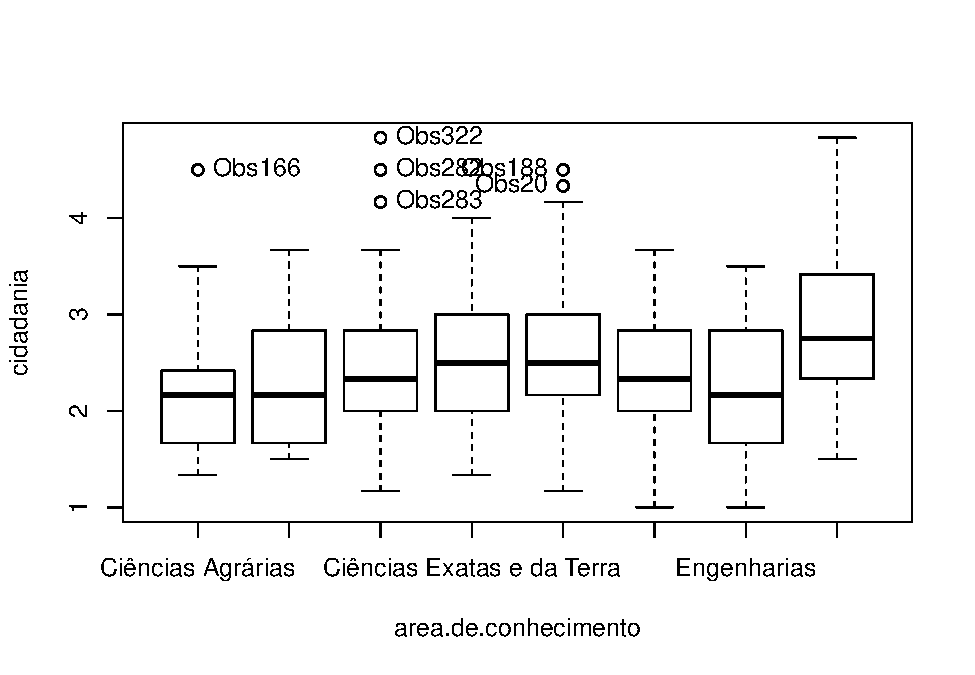
\includegraphics{factorialAnova_files/figure-latex/unnamed-chunk-3-1.pdf}

\begin{verbatim}
## [1] "Obs166" "Obs282" "Obs283" "Obs322" "Obs20"  "Obs188"
\end{verbatim}

\hypertarget{removing-outliers-from-the-data}{%
\subsubsection{Removing outliers from the
data}\label{removing-outliers-from-the-data}}

\begin{Shaded}
\begin{Highlighting}[]
\NormalTok{outliers <-}\StringTok{ }\KeywordTok{c}\NormalTok{(}\StringTok{"Obs20"}\NormalTok{,}\StringTok{"Obs160"}\NormalTok{,}\StringTok{"Obs166"}\NormalTok{,}\StringTok{"Obs188"}\NormalTok{,}\StringTok{"Obs282"}\NormalTok{,}\StringTok{"Obs283"}\NormalTok{,}\StringTok{"Obs322"}\NormalTok{)}
\NormalTok{rdat <-}\StringTok{ }\NormalTok{dat[}\OperatorTok{!}\NormalTok{dat[[}\StringTok{"ID"}\NormalTok{]] }\OperatorTok\StringTok{ }\NormalTok{outliers,]   }\CommentTok{# table without outliers}
\end{Highlighting}
\end{Shaded}

\begin{longtable}[]{@{}lllr@{}}
\caption{Outliers table}\tabularnewline
\toprule
& ID & area.de.conhecimento & cidadania\tabularnewline
\midrule
\endfirsthead
\toprule
& ID & area.de.conhecimento & cidadania\tabularnewline
\midrule
\endhead
Obs20 & Obs20 & Ciências Humanas & 4.333333\tabularnewline
Obs160 & Obs160 & Ciências Agrárias & 3.500000\tabularnewline
Obs166 & Obs166 & Ciências Agrárias & 4.500000\tabularnewline
Obs188 & Obs188 & Ciências Humanas & 4.500000\tabularnewline
Obs282 & Obs282 & Ciências da Saúde & 4.500000\tabularnewline
Obs283 & Obs283 & Ciências da Saúde & 4.166667\tabularnewline
Obs322 & Obs322 & Ciências da Saúde & 4.833333\tabularnewline
\bottomrule
\end{longtable}

\hypertarget{normality-assumption}{%
\subsubsection{Normality assumption}\label{normality-assumption}}

\textbf{Observation}:

As sample sizes increase, ANOVA remains a valid test even with the
violation of normality {[}\protect\hyperlink{references}{1},
\protect\hyperlink{references}{2}{]}. According to the central limit
theorem, the sampling distribution tends to be normal if the sample is
large enough (\texttt{n\ \textgreater{}\ 30}). Therefore, we performed
ANOVA with large samples as follows:

\begin{itemize}
\item
  In cases with the sample size greater than 30
  (\texttt{n\ \textgreater{}\ 30}), we adopted a significance level of
  \texttt{p\ \textless{}\ 0.01} instead a significance level of
  \texttt{p\ \textless{}\ 0.05}.
\item
  For samples with \texttt{n\ \textgreater{}\ 50} observation, we
  adopted D'Agostino-Pearson test that offers better accuracy for larger
  samples {[}\protect\hyperlink{references}{3}{]}.
\item
  For samples' size between \texttt{n\ \textgreater{}\ 100} and
  \texttt{n\ \textless{}=\ 200}, we ignored both tests (Shapiro and
  D'Agostino-Persons), and our decision of normality were based only in
  the interpretation of QQ-plots and histograms because these tests tend
  to be too sensitive with values greater than 200
  {[}\protect\hyperlink{references}{3}{]}.
\item
  For samples with \texttt{n\ \textgreater{}\ 200} observation, we
  ignore the normality assumption based on the central theorem limit,
  and taking only into account the homogeneity assumption.
\end{itemize}

\hypertarget{checking-normality-assumption-in-the-residual-model}{%
\paragraph{Checking normality assumption in the residual
model}\label{checking-normality-assumption-in-the-residual-model}}

\begin{Shaded}
\begin{Highlighting}[]
\NormalTok{mdl <-}\StringTok{ }\KeywordTok{lm}\NormalTok{(}\StringTok{`}\DataTypeTok{cidadania}\StringTok{`} \OperatorTok{~}\StringTok{ `}\DataTypeTok{area.de.conhecimento}\StringTok{`}\NormalTok{, }\DataTypeTok{data =}\NormalTok{ rdat)}
\KeywordTok{normality_test}\NormalTok{(}\KeywordTok{residuals}\NormalTok{(mdl))}
\end{Highlighting}
\end{Shaded}

\begin{verbatim}
##     n statistic     method          p p.signif normality
## 1 317   6.10095 D'Agostino 0.04733643       ns         -
\end{verbatim}

The QQ plot used to evaluate normality assumption

\begin{Shaded}
\begin{Highlighting}[]
\KeywordTok{qqPlot}\NormalTok{(}\KeywordTok{residuals}\NormalTok{(mdl))}
\end{Highlighting}
\end{Shaded}

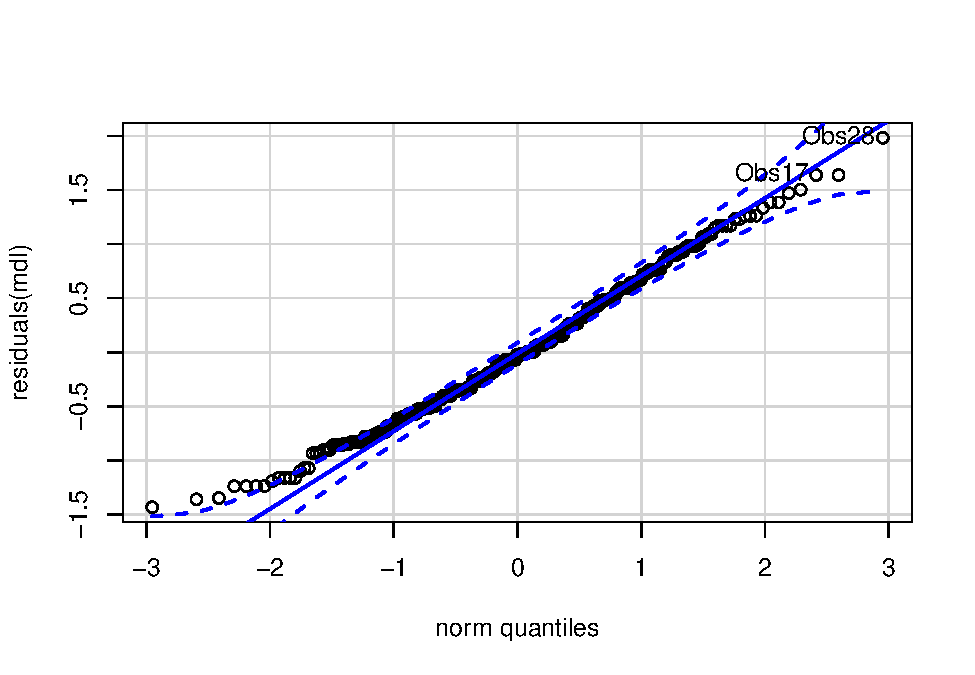
\includegraphics{factorialAnova_files/figure-latex/unnamed-chunk-7-1.pdf}

\begin{verbatim}
## Obs28 Obs17 
##    25    15
\end{verbatim}

\hypertarget{checking-normality-assumption-for-each-group}{%
\paragraph{Checking normality assumption for each
group}\label{checking-normality-assumption-for-each-group}}

\begin{Shaded}
\begin{Highlighting}[]
\KeywordTok{normality_test_at}\NormalTok{(}\KeywordTok{group_by}\NormalTok{(rdat, }\StringTok{`}\DataTypeTok{area.de.conhecimento}\StringTok{`}\NormalTok{), }\StringTok{"cidadania"}\NormalTok{)}
\end{Highlighting}
\end{Shaded}

\begin{verbatim}
##                 variable       area.de.conhecimento  n statistic
## 1              cidadania          Ciências Agrárias 26 0.9402270
## 2              cidadania        Ciências Biológicas 22 0.9053438
## Omnibus  Test  cidadania          Ciências da Saúde 62 0.1232339
## 11             cidadania Ciências Exatas e da Terra 48 0.9582129
## 12             cidadania           Ciências Humanas 43 0.9648051
## Omnibus  Test1 cidadania Ciências Sociais Aplicadas 53 1.1306457
## 13             cidadania                Engenharias 31 0.9617330
## 14             cidadania Linguística/Letras e Artes 32 0.9480897
##                      method          p p.signif normality
## 1              Shapiro-Wilk 0.13599788       ns       YES
## 2              Shapiro-Wilk 0.03807448        *        NO
## Omnibus  Test    D'Agostino 0.94024297       ns       YES
## 11             Shapiro-Wilk 0.08548516       ns       YES
## 12             Shapiro-Wilk 0.20727100       ns       YES
## Omnibus  Test1   D'Agostino 0.56817669       ns       YES
## 13             Shapiro-Wilk 0.32402466       ns       YES
## 14             Shapiro-Wilk 0.12718163       ns       YES
\end{verbatim}

\begin{itemize}
\tightlist
\item
  QQ plot in the \textbf{area.de.conhecimento}: ``Ciências Agrárias''
\end{itemize}

\begin{Shaded}
\begin{Highlighting}[]
\KeywordTok{qqPlot}\NormalTok{( }\OperatorTok{~}\StringTok{ `}\DataTypeTok{cidadania}\StringTok{`}\NormalTok{, }\DataTypeTok{data =}\NormalTok{ rdat[}\KeywordTok{which}\NormalTok{(rdat[}\StringTok{"area.de.conhecimento"}\NormalTok{] }\OperatorTok{==}\StringTok{ "Ciências Agrárias"}\NormalTok{),])}
\end{Highlighting}
\end{Shaded}

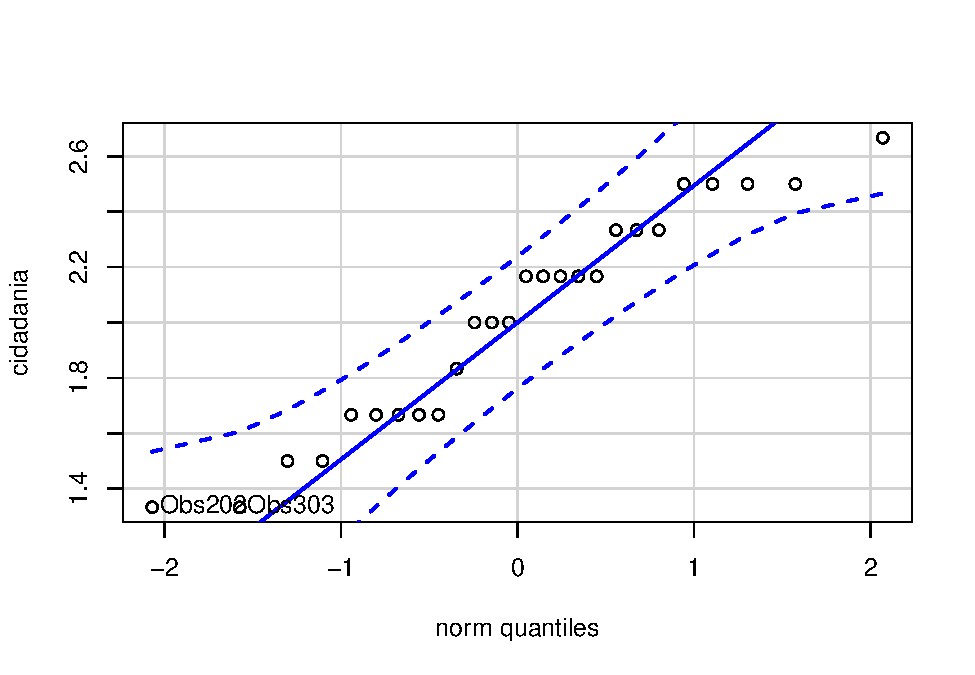
\includegraphics{factorialAnova_files/figure-latex/unnamed-chunk-9-1.pdf}

\begin{verbatim}
## Obs202 Obs303 
##     19     24
\end{verbatim}

\begin{itemize}
\tightlist
\item
  QQ plot in the \textbf{area.de.conhecimento}: ``Ciências Biológicas''
\end{itemize}

\begin{Shaded}
\begin{Highlighting}[]
\KeywordTok{qqPlot}\NormalTok{( }\OperatorTok{~}\StringTok{ `}\DataTypeTok{cidadania}\StringTok{`}\NormalTok{, }\DataTypeTok{data =}\NormalTok{ rdat[}\KeywordTok{which}\NormalTok{(rdat[}\StringTok{"area.de.conhecimento"}\NormalTok{] }\OperatorTok{==}\StringTok{ "Ciências Biológicas"),])}
\end{Highlighting}
\end{Shaded}

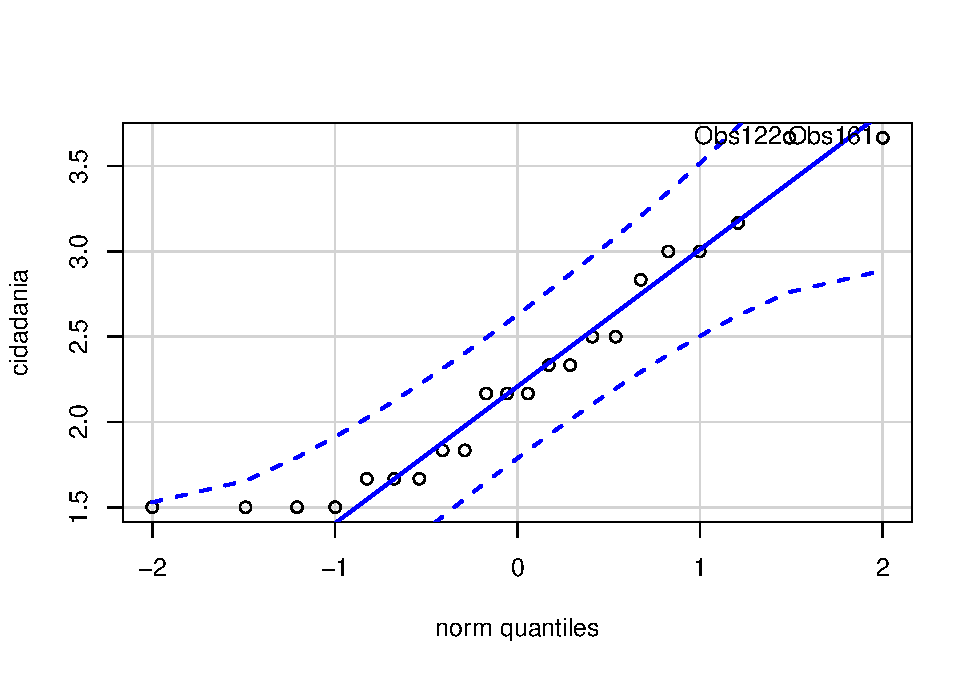
\includegraphics{factorialAnova_files/figure-latex/unnamed-chunk-10-1.pdf}

\begin{verbatim}
## Obs122 Obs161 
##      6     10
\end{verbatim}

\begin{itemize}
\tightlist
\item
  QQ plot in the \textbf{area.de.conhecimento}: ``Ciências da Saúde''
\end{itemize}

\begin{Shaded}
\begin{Highlighting}[]
\KeywordTok{qqPlot}\NormalTok{( }\OperatorTok{~}\StringTok{ `}\DataTypeTok{cidadania}\StringTok{`}\NormalTok{, }\DataTypeTok{data =}\NormalTok{ rdat[}\KeywordTok{which}\NormalTok{(rdat[}\StringTok{"area.de.conhecimento"}\NormalTok{] }\OperatorTok{==}\StringTok{ "Ciências da Saúde"),])}
\end{Highlighting}
\end{Shaded}

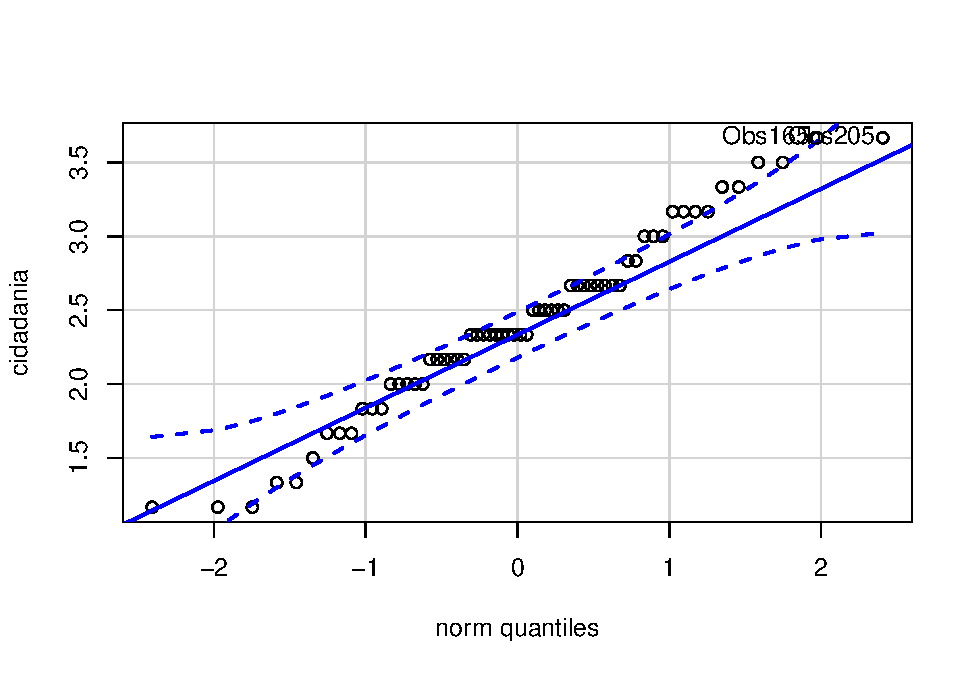
\includegraphics{factorialAnova_files/figure-latex/unnamed-chunk-11-1.pdf}

\begin{verbatim}
## Obs165 Obs205 
##     23     35
\end{verbatim}

\begin{itemize}
\tightlist
\item
  QQ plot in the \textbf{area.de.conhecimento}: ``Ciências Exatas e da
  Terra''
\end{itemize}

\begin{Shaded}
\begin{Highlighting}[]
\KeywordTok{qqPlot}\NormalTok{( }\OperatorTok{~}\StringTok{ `}\DataTypeTok{cidadania}\StringTok{`}\NormalTok{, }\DataTypeTok{data =}\NormalTok{ rdat[}\KeywordTok{which}\NormalTok{(rdat[}\StringTok{"area.de.conhecimento"}\NormalTok{] }\OperatorTok{==}\StringTok{ "Ciências Exatas e da Terra"}\NormalTok{),])}
\end{Highlighting}
\end{Shaded}

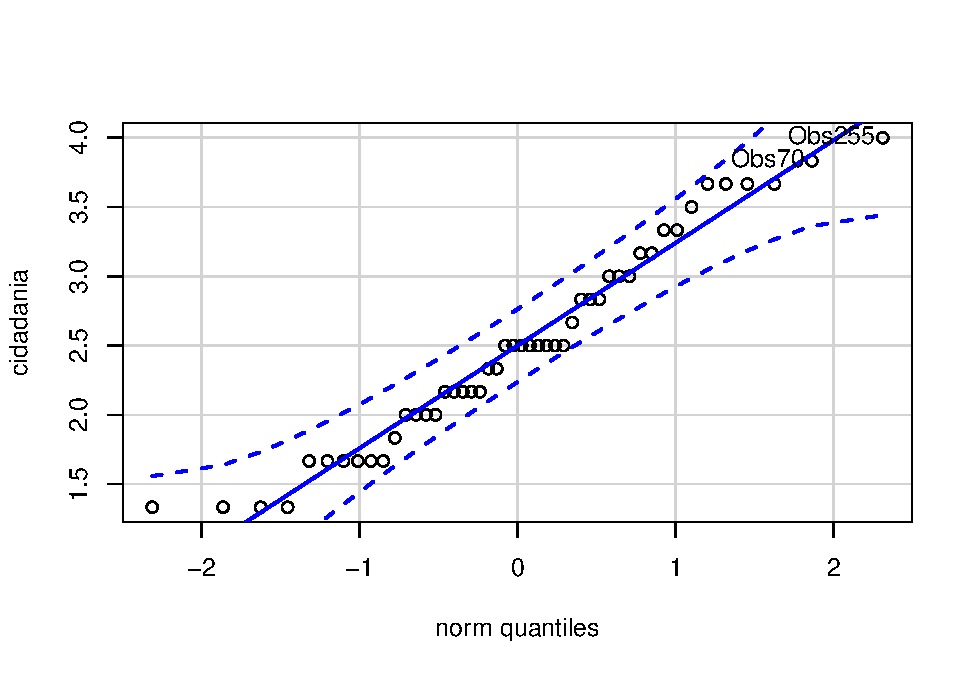
\includegraphics{factorialAnova_files/figure-latex/unnamed-chunk-12-1.pdf}

\begin{verbatim}
## Obs255  Obs70 
##     36     11
\end{verbatim}

\begin{itemize}
\tightlist
\item
  QQ plot in the \textbf{area.de.conhecimento}: ``Ciências Humanas''
\end{itemize}

\begin{Shaded}
\begin{Highlighting}[]
\KeywordTok{qqPlot}\NormalTok{( }\OperatorTok{~}\StringTok{ `}\DataTypeTok{cidadania}\StringTok{`}\NormalTok{, }\DataTypeTok{data =}\NormalTok{ rdat[}\KeywordTok{which}\NormalTok{(rdat[}\StringTok{"area.de.conhecimento"}\NormalTok{] }\OperatorTok{==}\StringTok{ "Ciências Humanas"}\NormalTok{),])}
\end{Highlighting}
\end{Shaded}

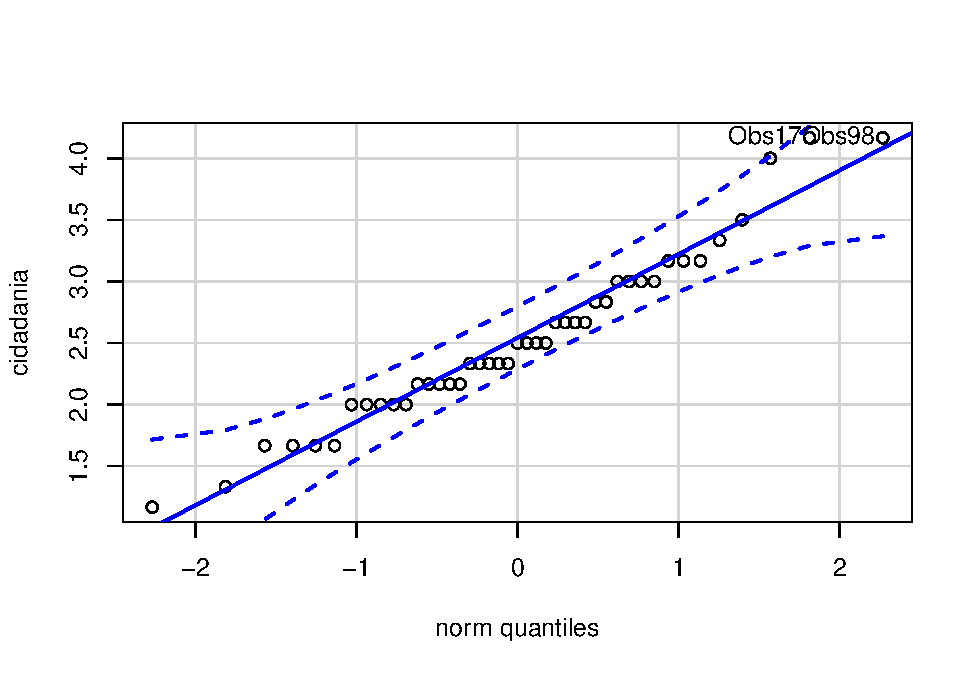
\includegraphics{factorialAnova_files/figure-latex/unnamed-chunk-13-1.pdf}

\begin{verbatim}
## Obs17 Obs98 
##     2    19
\end{verbatim}

\begin{itemize}
\tightlist
\item
  QQ plot in the \textbf{area.de.conhecimento}: ``Ciências Sociais
  Aplicadas''
\end{itemize}

\begin{Shaded}
\begin{Highlighting}[]
\KeywordTok{qqPlot}\NormalTok{( }\OperatorTok{~}\StringTok{ `}\DataTypeTok{cidadania}\StringTok{`}\NormalTok{, }\DataTypeTok{data =}\NormalTok{ rdat[}\KeywordTok{which}\NormalTok{(rdat[}\StringTok{"area.de.conhecimento"}\NormalTok{] }\OperatorTok{==}\StringTok{ "Ciências Sociais Aplicadas"}\NormalTok{),])}
\end{Highlighting}
\end{Shaded}

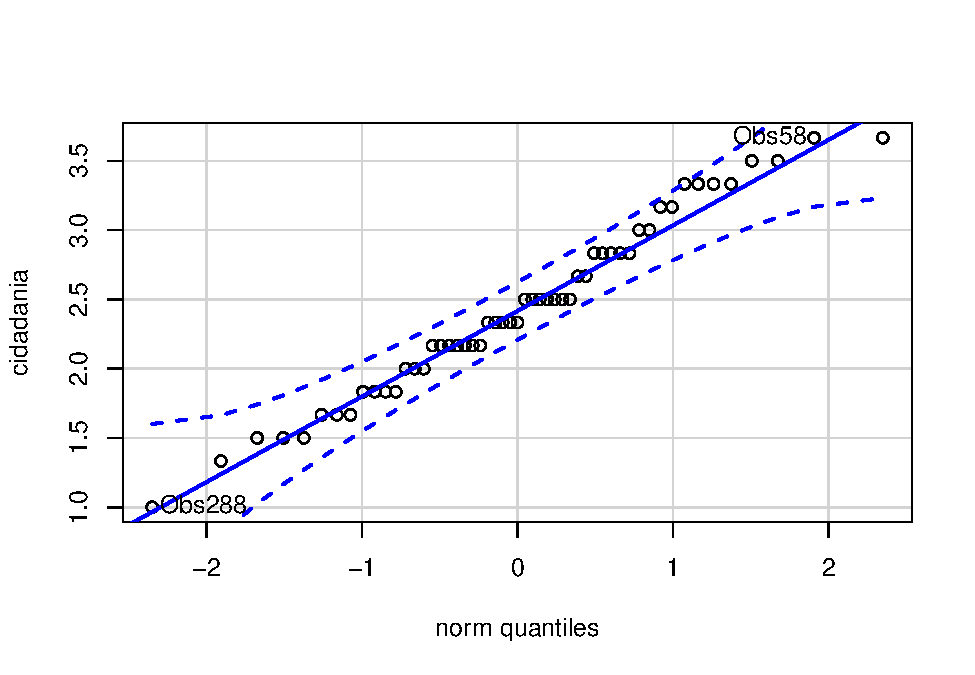
\includegraphics{factorialAnova_files/figure-latex/unnamed-chunk-14-1.pdf}

\begin{verbatim}
## Obs288  Obs58 
##     46     18
\end{verbatim}

\begin{itemize}
\tightlist
\item
  QQ plot in the \textbf{area.de.conhecimento}: ``Engenharias''
\end{itemize}

\begin{Shaded}
\begin{Highlighting}[]
\KeywordTok{qqPlot}\NormalTok{( }\OperatorTok{~}\StringTok{ `}\DataTypeTok{cidadania}\StringTok{`}\NormalTok{, }\DataTypeTok{data =}\NormalTok{ rdat[}\KeywordTok{which}\NormalTok{(rdat[}\StringTok{"area.de.conhecimento"}\NormalTok{] }\OperatorTok{==}\StringTok{ "Engenharias"}\NormalTok{),])}
\end{Highlighting}
\end{Shaded}

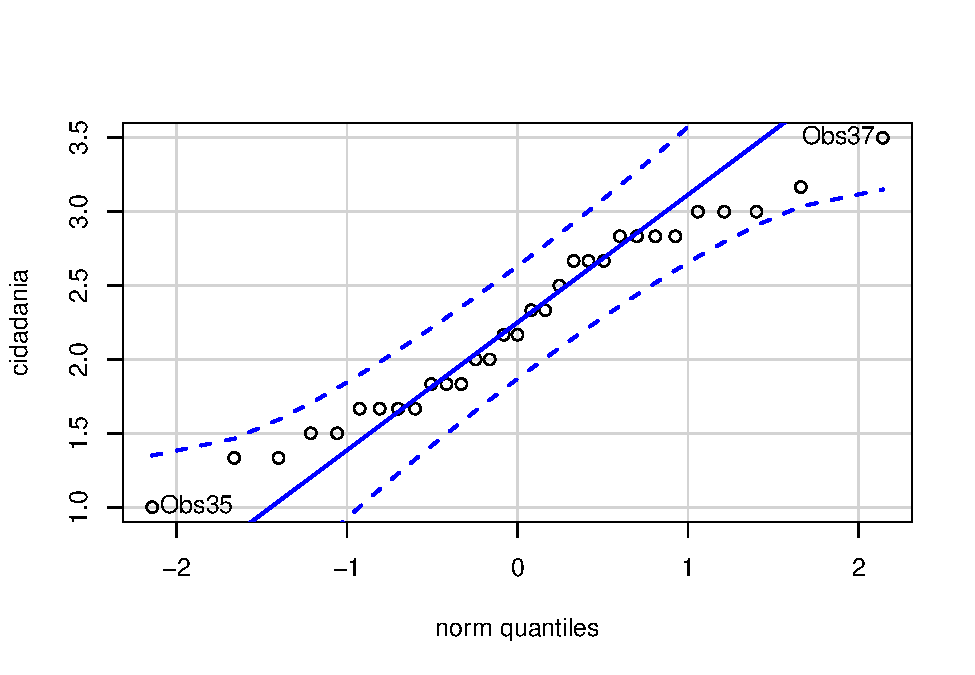
\includegraphics{factorialAnova_files/figure-latex/unnamed-chunk-15-1.pdf}

\begin{verbatim}
## Obs37 Obs35 
##     4     2
\end{verbatim}

\begin{itemize}
\tightlist
\item
  QQ plot in the \textbf{area.de.conhecimento}: ``Linguística/Letras e
  Artes''
\end{itemize}

\begin{Shaded}
\begin{Highlighting}[]
\KeywordTok{qqPlot}\NormalTok{( }\OperatorTok{~}\StringTok{ `}\DataTypeTok{cidadania}\StringTok{`}\NormalTok{, }\DataTypeTok{data =}\NormalTok{ rdat[}\KeywordTok{which}\NormalTok{(rdat[}\StringTok{"area.de.conhecimento"}\NormalTok{] }\OperatorTok{==}\StringTok{ "Linguística/Letras e Artes"}\NormalTok{),])}
\end{Highlighting}
\end{Shaded}

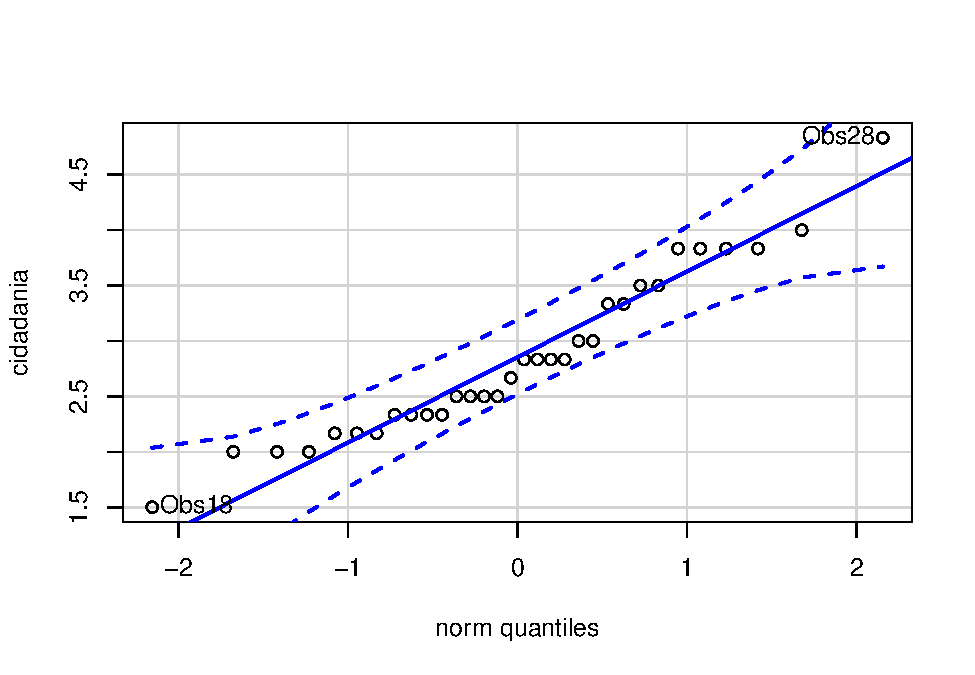
\includegraphics{factorialAnova_files/figure-latex/unnamed-chunk-16-1.pdf}

\begin{verbatim}
## Obs28 Obs18 
##     3     2
\end{verbatim}

\hypertarget{removing-data-that-affect-normality}{%
\paragraph{Removing data that affect
normality}\label{removing-data-that-affect-normality}}

\begin{Shaded}
\begin{Highlighting}[]
\NormalTok{non.normal <-}\StringTok{ }\KeywordTok{c}\NormalTok{(}\StringTok{"Obs133"}\NormalTok{)}
\NormalTok{sdat <-}\StringTok{ }\NormalTok{rdat[}\OperatorTok{!}\NormalTok{rdat[[}\StringTok{"ID"}\NormalTok{]] }\OperatorTok\StringTok{ }\NormalTok{non.normal,]   }\CommentTok{# table without non-normal and outliers}
\end{Highlighting}
\end{Shaded}

\begin{longtable}[]{@{}lllr@{}}
\caption{Non-normal data table}\tabularnewline
\toprule
& ID & area.de.conhecimento & cidadania\tabularnewline
\midrule
\endfirsthead
\toprule
& ID & area.de.conhecimento & cidadania\tabularnewline
\midrule
\endhead
Obs133 & Obs133 & Ciências Biológicas & 1.5\tabularnewline
\bottomrule
\end{longtable}

\hypertarget{performing-normality-test-without-data-that-affect-normality}{%
\paragraph{Performing normality test without data that affect
normality}\label{performing-normality-test-without-data-that-affect-normality}}

\begin{Shaded}
\begin{Highlighting}[]
\NormalTok{mdl <-}\StringTok{ }\KeywordTok{lm}\NormalTok{(}\StringTok{`}\DataTypeTok{cidadania}\StringTok{`} \OperatorTok{~}\StringTok{ `}\DataTypeTok{area.de.conhecimento}\StringTok{`}\NormalTok{, }\DataTypeTok{data =}\NormalTok{ sdat)}
\KeywordTok{normality_test}\NormalTok{(}\KeywordTok{residuals}\NormalTok{(mdl))}
\end{Highlighting}
\end{Shaded}

\begin{longtable}[]{@{}rrllll@{}}
\toprule
n & statistic & method & p & p.signif & normality\tabularnewline
\midrule
\endhead
316 & 5.9405 & D'Agostino & 0.0513 & ns & -\tabularnewline
\bottomrule
\end{longtable}

\begin{Shaded}
\begin{Highlighting}[]
\KeywordTok{normality_test_at}\NormalTok{(}\KeywordTok{group_by}\NormalTok{(sdat, }\StringTok{`}\DataTypeTok{area.de.conhecimento}\StringTok{`}\NormalTok{), }\StringTok{"cidadania"}\NormalTok{)}
\end{Highlighting}
\end{Shaded}

\begin{longtable}[]{@{}llrrllll@{}}
\toprule
variable & area.de.conhecimento & n & statistic & method & p & p.signif
& normality\tabularnewline
\midrule
\endhead
cidadania & Ciências Agrárias & 26 & 0.9402 & Shapiro-Wilk & 0.136 & ns
& YES\tabularnewline
cidadania & Ciências Biológicas & 21 & 0.9161 & Shapiro-Wilk & 0.0724 &
ns & YES\tabularnewline
cidadania & Ciências da Saúde & 62 & 0.1232 & D'Agostino & 0.9402 & ns &
YES\tabularnewline
cidadania & Ciências Exatas e da Terra & 48 & 0.9582 & Shapiro-Wilk &
0.0855 & ns & YES\tabularnewline
cidadania & Ciências Humanas & 43 & 0.9648 & Shapiro-Wilk & 0.2073 & ns
& YES\tabularnewline
cidadania & Ciências Sociais Aplicadas & 53 & 1.1306 & D'Agostino &
0.5682 & ns & YES\tabularnewline
cidadania & Engenharias & 31 & 0.9617 & Shapiro-Wilk & 0.324 & ns &
YES\tabularnewline
cidadania & Linguística/Letras e Artes & 32 & 0.9481 & Shapiro-Wilk &
0.1272 & ns & YES\tabularnewline
\bottomrule
\end{longtable}

QQ plot in the residual model without data that affect normality

\begin{Shaded}
\begin{Highlighting}[]
\KeywordTok{qqPlot}\NormalTok{(}\KeywordTok{residuals}\NormalTok{(mdl))}
\end{Highlighting}
\end{Shaded}

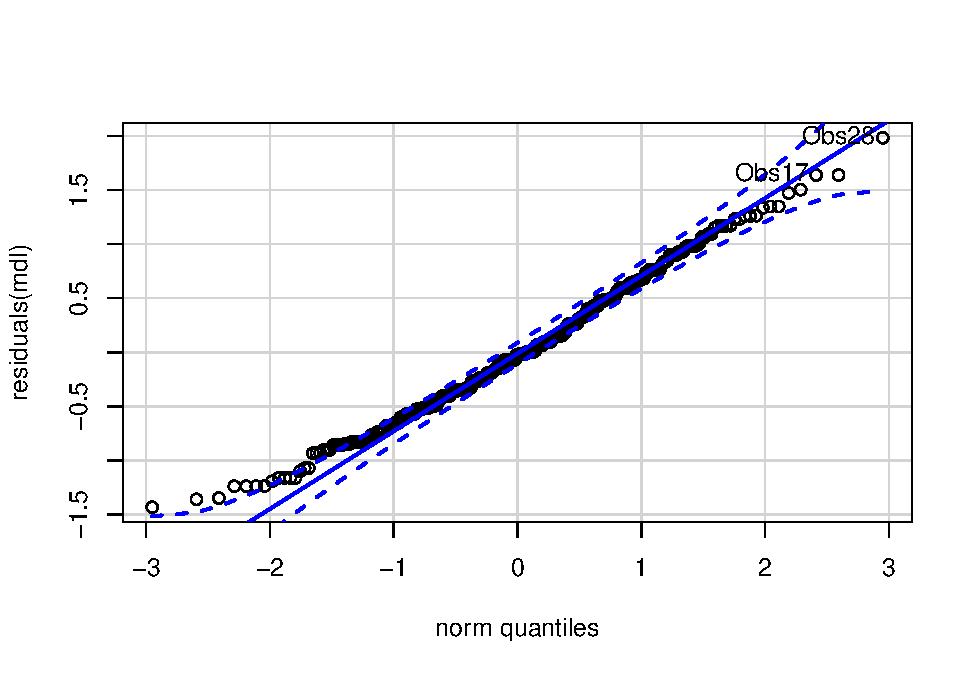
\includegraphics{factorialAnova_files/figure-latex/unnamed-chunk-21-1.pdf}

\begin{verbatim}
## Obs28 Obs17 
##    25    15
\end{verbatim}

\begin{itemize}
\tightlist
\item
  QQ plot in the \textbf{area.de.conhecimento}: ``Ciências Agrárias''
\end{itemize}

\begin{Shaded}
\begin{Highlighting}[]
\KeywordTok{qqPlot}\NormalTok{( }\OperatorTok{~}\StringTok{ `}\DataTypeTok{cidadania}\StringTok{`}\NormalTok{, }\DataTypeTok{data =}\NormalTok{ sdat[}\KeywordTok{which}\NormalTok{(sdat[}\StringTok{"area.de.conhecimento"}\NormalTok{] }\OperatorTok{==}\StringTok{ "Ciências Agrárias"}\NormalTok{),])}
\end{Highlighting}
\end{Shaded}

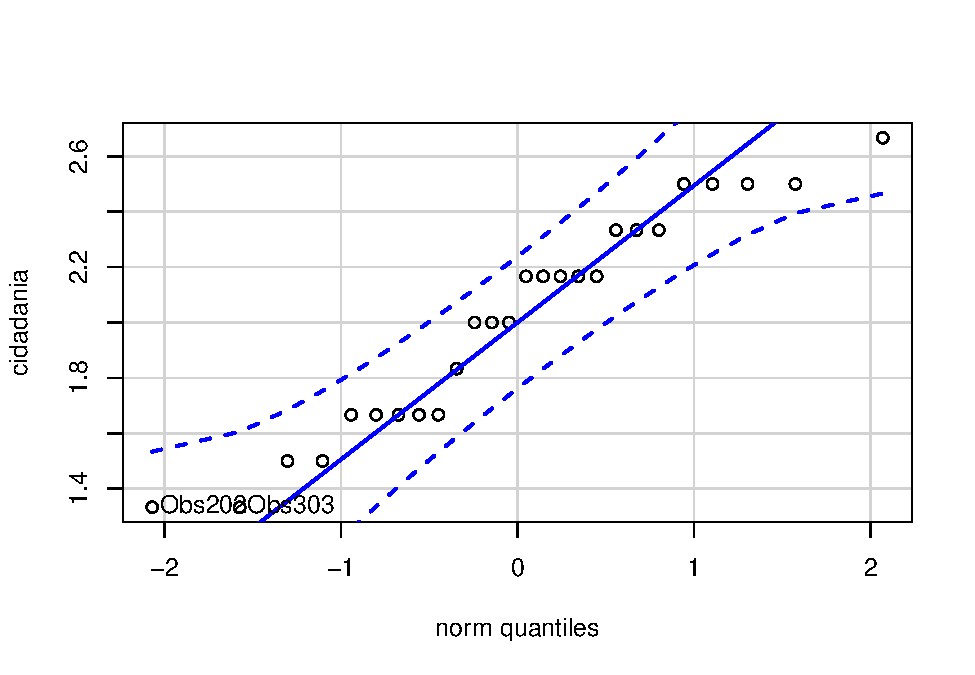
\includegraphics{factorialAnova_files/figure-latex/unnamed-chunk-22-1.pdf}

\begin{verbatim}
## Obs202 Obs303 
##     19     24
\end{verbatim}

\begin{itemize}
\tightlist
\item
  QQ plot in the \textbf{area.de.conhecimento}: ``Ciências Biológicas''
\end{itemize}

\begin{Shaded}
\begin{Highlighting}[]
\KeywordTok{qqPlot}\NormalTok{( }\OperatorTok{~}\StringTok{ `}\DataTypeTok{cidadania}\StringTok{`}\NormalTok{, }\DataTypeTok{data =}\NormalTok{ sdat[}\KeywordTok{which}\NormalTok{(sdat[}\StringTok{"area.de.conhecimento"}\NormalTok{] }\OperatorTok{==}\StringTok{ "Ciências Biológicas"),])}
\end{Highlighting}
\end{Shaded}

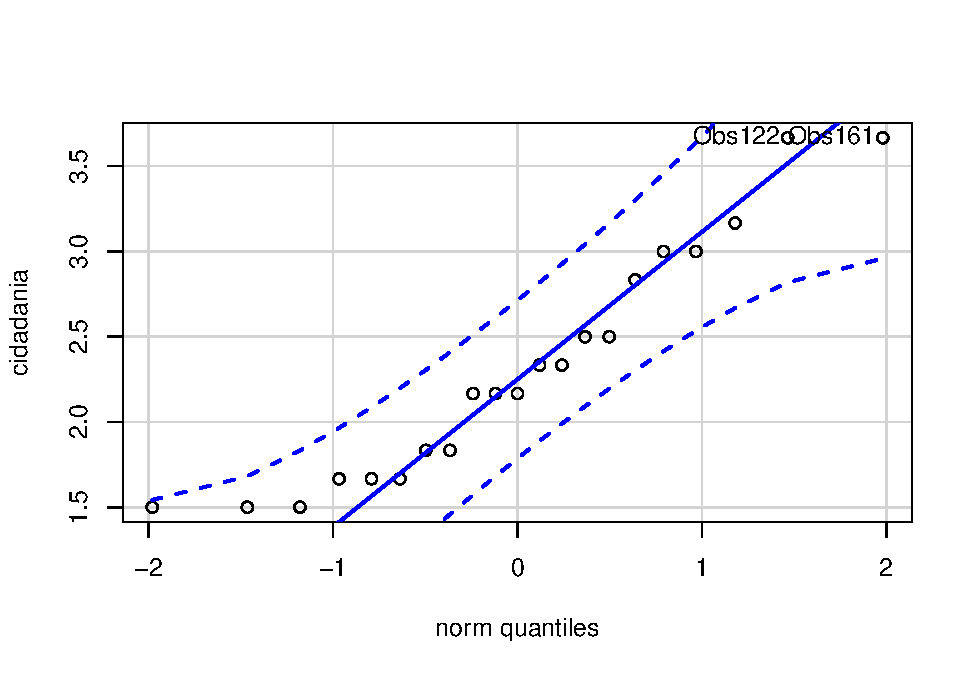
\includegraphics{factorialAnova_files/figure-latex/unnamed-chunk-23-1.pdf}

\begin{verbatim}
## Obs122 Obs161 
##      6      9
\end{verbatim}

\begin{itemize}
\tightlist
\item
  QQ plot in the \textbf{area.de.conhecimento}: ``Ciências da Saúde''
\end{itemize}

\begin{Shaded}
\begin{Highlighting}[]
\KeywordTok{qqPlot}\NormalTok{( }\OperatorTok{~}\StringTok{ `}\DataTypeTok{cidadania}\StringTok{`}\NormalTok{, }\DataTypeTok{data =}\NormalTok{ sdat[}\KeywordTok{which}\NormalTok{(sdat[}\StringTok{"area.de.conhecimento"}\NormalTok{] }\OperatorTok{==}\StringTok{ "Ciências da Saúde"),])}
\end{Highlighting}
\end{Shaded}

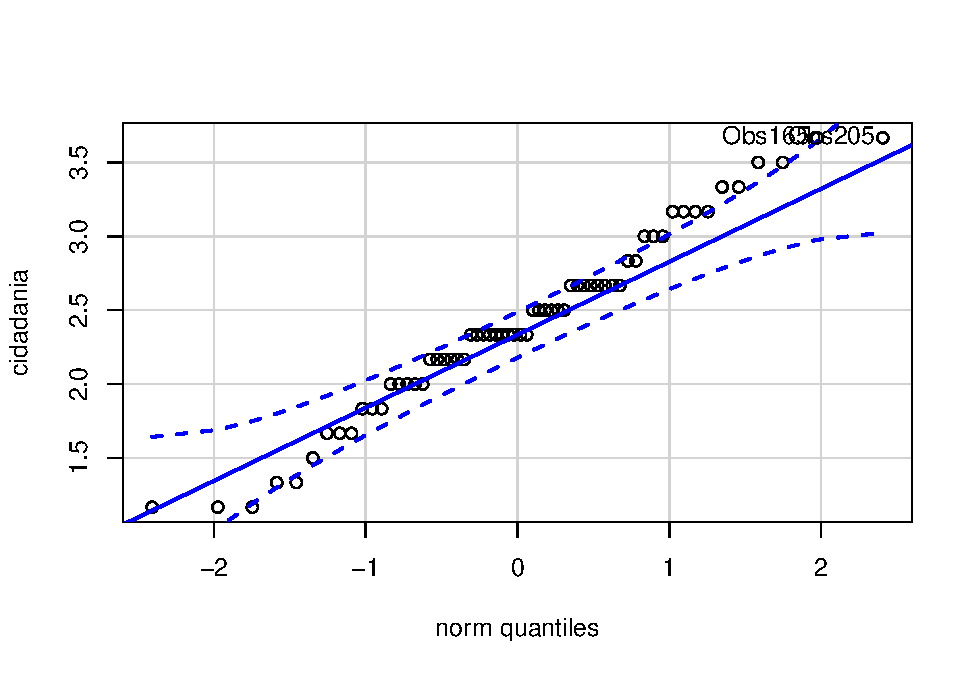
\includegraphics{factorialAnova_files/figure-latex/unnamed-chunk-24-1.pdf}

\begin{verbatim}
## Obs165 Obs205 
##     23     35
\end{verbatim}

\begin{itemize}
\tightlist
\item
  QQ plot in the \textbf{area.de.conhecimento}: ``Ciências Exatas e da
  Terra''
\end{itemize}

\begin{Shaded}
\begin{Highlighting}[]
\KeywordTok{qqPlot}\NormalTok{( }\OperatorTok{~}\StringTok{ `}\DataTypeTok{cidadania}\StringTok{`}\NormalTok{, }\DataTypeTok{data =}\NormalTok{ sdat[}\KeywordTok{which}\NormalTok{(sdat[}\StringTok{"area.de.conhecimento"}\NormalTok{] }\OperatorTok{==}\StringTok{ "Ciências Exatas e da Terra"}\NormalTok{),])}
\end{Highlighting}
\end{Shaded}

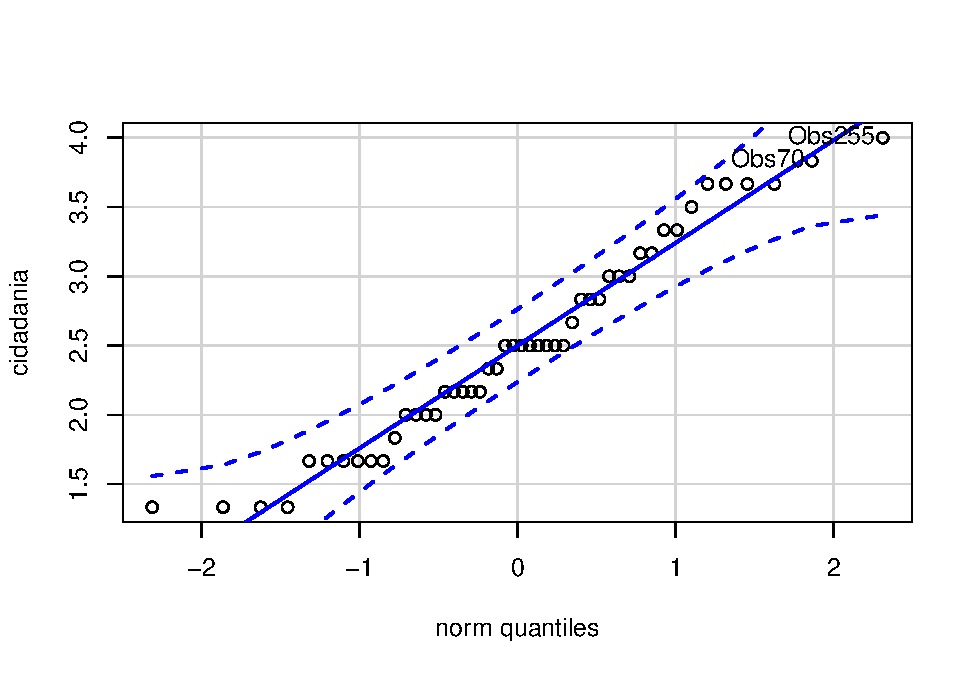
\includegraphics{factorialAnova_files/figure-latex/unnamed-chunk-25-1.pdf}

\begin{verbatim}
## Obs255  Obs70 
##     36     11
\end{verbatim}

\begin{itemize}
\tightlist
\item
  QQ plot in the \textbf{area.de.conhecimento}: ``Ciências Humanas''
\end{itemize}

\begin{Shaded}
\begin{Highlighting}[]
\KeywordTok{qqPlot}\NormalTok{( }\OperatorTok{~}\StringTok{ `}\DataTypeTok{cidadania}\StringTok{`}\NormalTok{, }\DataTypeTok{data =}\NormalTok{ sdat[}\KeywordTok{which}\NormalTok{(sdat[}\StringTok{"area.de.conhecimento"}\NormalTok{] }\OperatorTok{==}\StringTok{ "Ciências Humanas"}\NormalTok{),])}
\end{Highlighting}
\end{Shaded}

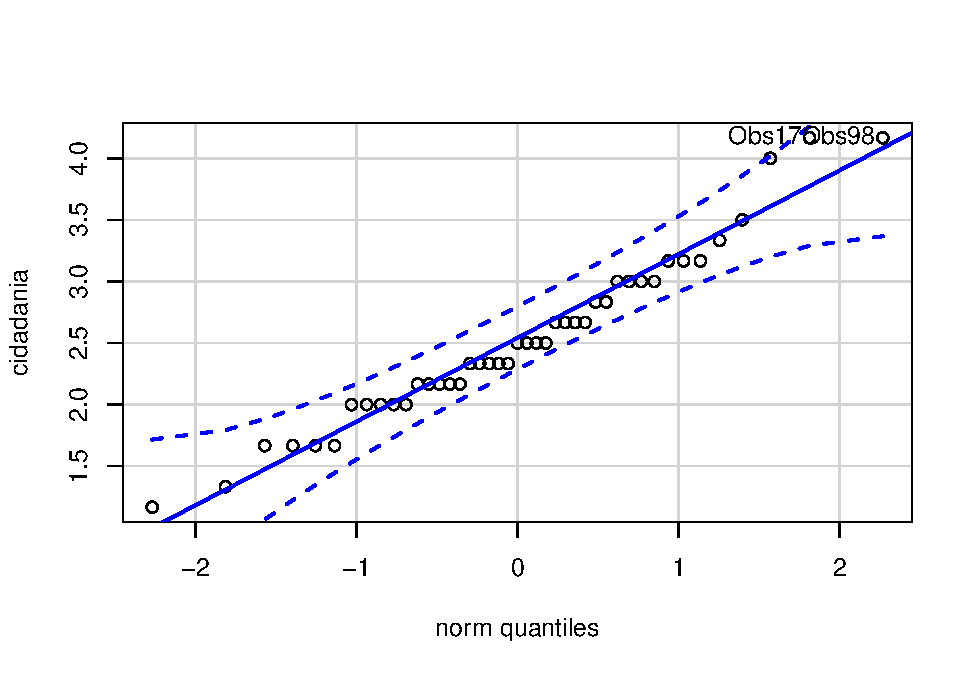
\includegraphics{factorialAnova_files/figure-latex/unnamed-chunk-26-1.pdf}

\begin{verbatim}
## Obs17 Obs98 
##     2    19
\end{verbatim}

\begin{itemize}
\tightlist
\item
  QQ plot in the \textbf{area.de.conhecimento}: ``Ciências Sociais
  Aplicadas''
\end{itemize}

\begin{Shaded}
\begin{Highlighting}[]
\KeywordTok{qqPlot}\NormalTok{( }\OperatorTok{~}\StringTok{ `}\DataTypeTok{cidadania}\StringTok{`}\NormalTok{, }\DataTypeTok{data =}\NormalTok{ sdat[}\KeywordTok{which}\NormalTok{(sdat[}\StringTok{"area.de.conhecimento"}\NormalTok{] }\OperatorTok{==}\StringTok{ "Ciências Sociais Aplicadas"}\NormalTok{),])}
\end{Highlighting}
\end{Shaded}

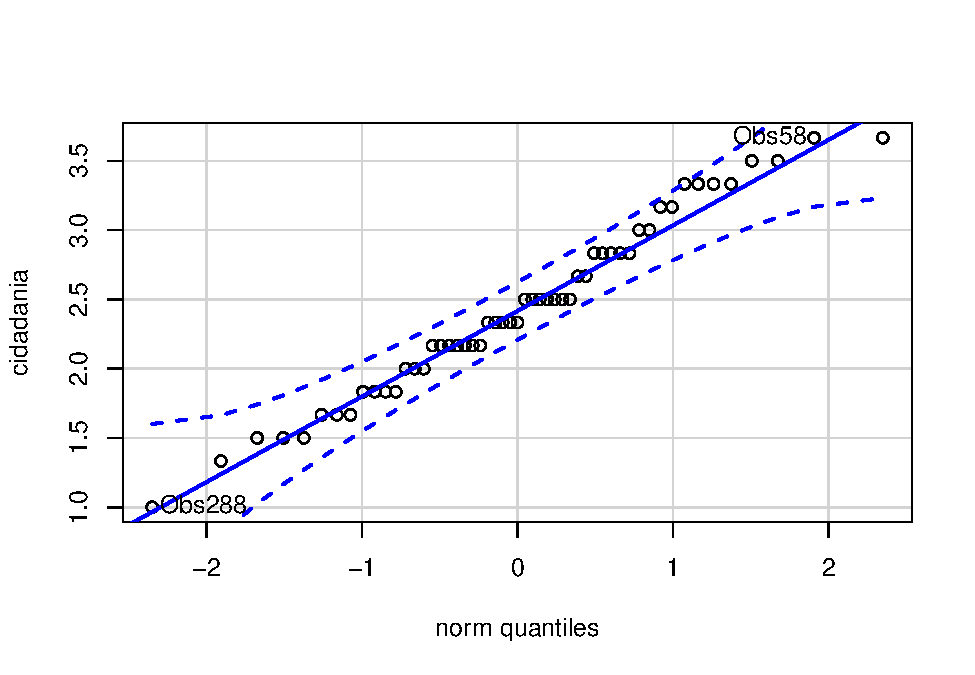
\includegraphics{factorialAnova_files/figure-latex/unnamed-chunk-27-1.pdf}

\begin{verbatim}
## Obs288  Obs58 
##     46     18
\end{verbatim}

\begin{itemize}
\tightlist
\item
  QQ plot in the \textbf{area.de.conhecimento}: ``Engenharias''
\end{itemize}

\begin{Shaded}
\begin{Highlighting}[]
\KeywordTok{qqPlot}\NormalTok{( }\OperatorTok{~}\StringTok{ `}\DataTypeTok{cidadania}\StringTok{`}\NormalTok{, }\DataTypeTok{data =}\NormalTok{ sdat[}\KeywordTok{which}\NormalTok{(sdat[}\StringTok{"area.de.conhecimento"}\NormalTok{] }\OperatorTok{==}\StringTok{ "Engenharias"}\NormalTok{),])}
\end{Highlighting}
\end{Shaded}

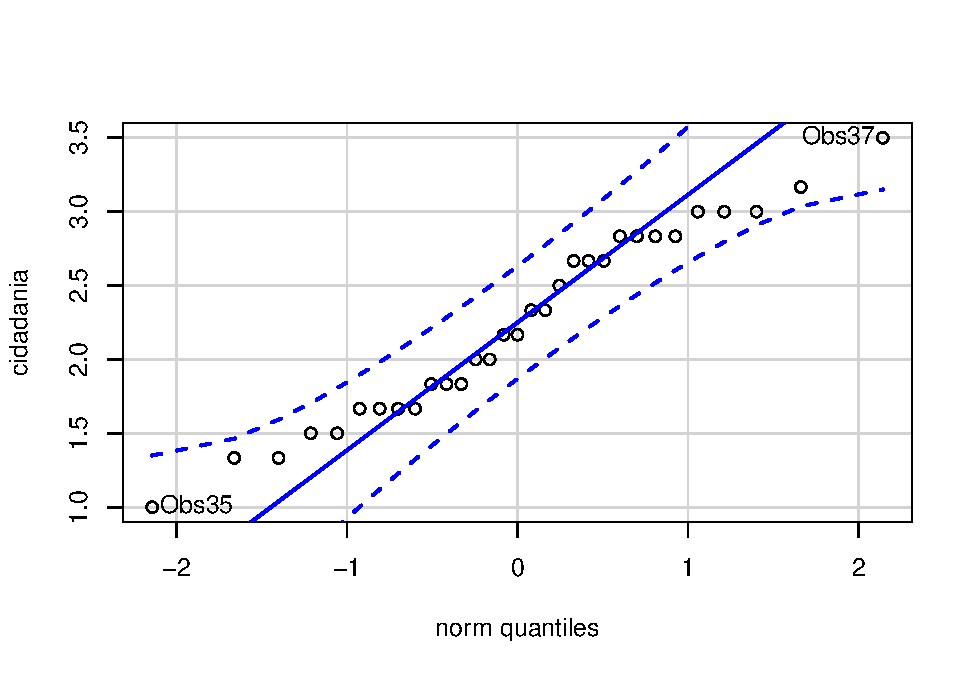
\includegraphics{factorialAnova_files/figure-latex/unnamed-chunk-28-1.pdf}

\begin{verbatim}
## Obs37 Obs35 
##     4     2
\end{verbatim}

\begin{itemize}
\tightlist
\item
  QQ plot in the \textbf{area.de.conhecimento}: ``Linguística/Letras e
  Artes''
\end{itemize}

\begin{Shaded}
\begin{Highlighting}[]
\KeywordTok{qqPlot}\NormalTok{( }\OperatorTok{~}\StringTok{ `}\DataTypeTok{cidadania}\StringTok{`}\NormalTok{, }\DataTypeTok{data =}\NormalTok{ sdat[}\KeywordTok{which}\NormalTok{(sdat[}\StringTok{"area.de.conhecimento"}\NormalTok{] }\OperatorTok{==}\StringTok{ "Linguística/Letras e Artes"}\NormalTok{),])}
\end{Highlighting}
\end{Shaded}

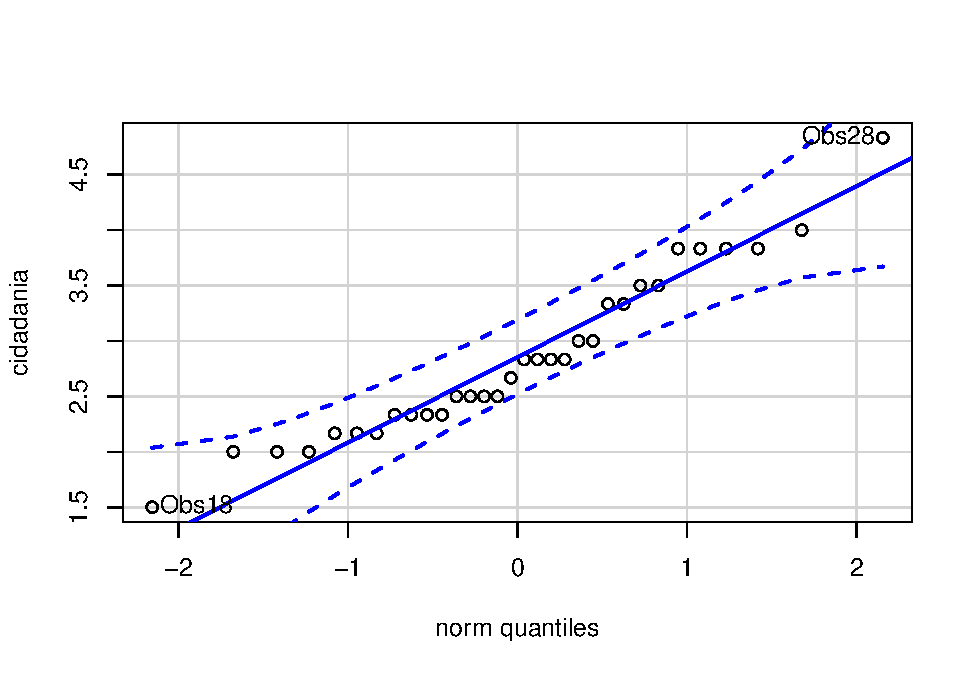
\includegraphics{factorialAnova_files/figure-latex/unnamed-chunk-29-1.pdf}

\begin{verbatim}
## Obs28 Obs18 
##     3     2
\end{verbatim}

\hypertarget{homogeneity-of-variance-assumption}{%
\subsubsection{Homogeneity of variance
assumption}\label{homogeneity-of-variance-assumption}}

\begin{Shaded}
\begin{Highlighting}[]
\KeywordTok{levene_test}\NormalTok{(sdat, }\StringTok{`}\DataTypeTok{cidadania}\StringTok{`} \OperatorTok{~}\StringTok{ `}\DataTypeTok{area.de.conhecimento}\StringTok{`}\NormalTok{)}
\end{Highlighting}
\end{Shaded}

\begin{longtable}[]{@{}rrrll@{}}
\toprule
df1 & df2 & statistic & p & p.signif\tabularnewline
\midrule
\endhead
7 & 308 & 1.417 & 0.1977 & ns\tabularnewline
\bottomrule
\end{longtable}

From the output above, non-significant difference indicates homogeneity
of variance in the different groups (Signif. codes: 0 **** 0.0001 ***
0.001 ** 0.01 * 0.05 ns 1).

\hypertarget{computation-anova}{%
\subsection{Computation ANOVA}\label{computation-anova}}

\begin{Shaded}
\begin{Highlighting}[]
\NormalTok{res.aov <-}\StringTok{ }\KeywordTok{anova_test}\NormalTok{(sdat, }\StringTok{`}\DataTypeTok{cidadania}\StringTok{`} \OperatorTok{~}\StringTok{ `}\DataTypeTok{area.de.conhecimento}\StringTok{`}\NormalTok{, }\DataTypeTok{type =} \DecValTok{2}\NormalTok{, }\DataTypeTok{effect.size =} \StringTok{'ges'}\NormalTok{, }\DataTypeTok{detailed =}\NormalTok{ T)}
\KeywordTok{get_anova_table}\NormalTok{(res.aov)}
\end{Highlighting}
\end{Shaded}

\begin{verbatim}
## Coefficient covariances computed by hccm()
\end{verbatim}

\begin{longtable}[]{@{}lrrrrrllr@{}}
\toprule
Effect & SSn & SSd & DFn & DFd & F & p & p\textless{}.05 &
ges\tabularnewline
\midrule
\endhead
area.de.conhecimento & 12.222 & 133.352 & 7 & 308 & 4.033 & 3e-04 & * &
0.084\tabularnewline
\bottomrule
\end{longtable}

\hypertarget{post-hoct-tests-pairwise-comparisons}{%
\subsection{Post-hoct Tests (Pairwise
Comparisons)}\label{post-hoct-tests-pairwise-comparisons}}

\begin{itemize}
\tightlist
\item
  Estimated marginal means for \textbf{area.de.conhecimento}
\end{itemize}

\begin{Shaded}
\begin{Highlighting}[]
\NormalTok{(emm[[}\StringTok{"area.de.conhecimento"}\NormalTok{]] <-}\StringTok{ }\KeywordTok{emmeans_test}\NormalTok{(sdat, }\StringTok{`}\DataTypeTok{cidadania}\StringTok{`} \OperatorTok{~}\StringTok{ `}\DataTypeTok{area.de.conhecimento}\StringTok{`}\NormalTok{, }\DataTypeTok{p.adjust.method =} \StringTok{"bonferroni"}\NormalTok{, }\DataTypeTok{detailed =}\NormalTok{ T))}
\end{Highlighting}
\end{Shaded}

\begin{longtable}[]{@{}lllrrrrrrrll@{}}
\toprule
.y. & group1 & group2 & estimate & se & df & conf.low & conf.high &
statistic & p & p.adj & p.adj.signif\tabularnewline
\midrule
\endhead
cidadania & Ciências Agrárias & Ciências Biológicas & -0.3046 & 0.1931 &
308 & -0.6845 & 0.0752 & -1.5780 & 0.1156 & 1 & ns\tabularnewline
cidadania & Ciências Agrárias & Ciências da Saúde & -0.3931 & 0.1537 &
308 & -0.6956 & -0.0906 & -2.5569 & 0.0110 & 0.3091 & ns\tabularnewline
cidadania & Ciências Agrárias & Ciências Exatas e da Terra & -0.4837 &
0.1602 & 308 & -0.7990 & -0.1684 & -3.0189 & 0.0027 & 0.077 &
ns\tabularnewline
cidadania & Ciências Agrárias & Ciências Humanas & -0.5143 & 0.1635 &
308 & -0.8360 & -0.1927 & -3.1463 & 0.0018 & 0.0508 & ns\tabularnewline
cidadania & Ciências Agrárias & Ciências Sociais Aplicadas & -0.4211 &
0.1575 & 308 & -0.7311 & -0.1111 & -2.6731 & 0.0079 & 0.2216 &
ns\tabularnewline
cidadania & Ciências Agrárias & Engenharias & -0.2237 & 0.1750 & 308 &
-0.5681 & 0.1206 & -1.2786 & 0.2020 & 1 & ns\tabularnewline
cidadania & Ciências Agrárias & Linguística/Letras e Artes & -0.8361 &
0.1737 & 308 & -1.1780 & -0.4943 & -4.8128 & 0.0000 & 1e-04 &
****\tabularnewline
cidadania & Ciências Biológicas & Ciências da Saúde & -0.0885 & 0.1661 &
308 & -0.4154 & 0.2384 & -0.5324 & 0.5948 & 1 & ns\tabularnewline
cidadania & Ciências Biológicas & Ciências Exatas e da Terra & -0.1791 &
0.1722 & 308 & -0.5178 & 0.1597 & -1.0402 & 0.2991 & 1 &
ns\tabularnewline
cidadania & Ciências Biológicas & Ciências Humanas & -0.2097 & 0.1752 &
308 & -0.5544 & 0.1350 & -1.1969 & 0.2323 & 1 & ns\tabularnewline
cidadania & Ciências Biológicas & Ciências Sociais Aplicadas & -0.1165 &
0.1697 & 308 & -0.4504 & 0.2173 & -0.6867 & 0.4928 & 1 &
ns\tabularnewline
cidadania & Ciências Biológicas & Engenharias & 0.0809 & 0.1860 & 308 &
-0.2850 & 0.4468 & 0.4350 & 0.6638 & 1 & ns\tabularnewline
cidadania & Ciências Biológicas & Linguística/Letras e Artes & -0.5315 &
0.1848 & 308 & -0.8951 & -0.1679 & -2.8762 & 0.0043 & 0.1205 &
ns\tabularnewline
cidadania & Ciências da Saúde & Ciências Exatas e da Terra & -0.0906 &
0.1265 & 308 & -0.3395 & 0.1583 & -0.7163 & 0.4744 & 1 &
ns\tabularnewline
cidadania & Ciências da Saúde & Ciências Humanas & -0.1212 & 0.1306 &
308 & -0.3782 & 0.1357 & -0.9283 & 0.3540 & 1 & ns\tabularnewline
cidadania & Ciências da Saúde & Ciências Sociais Aplicadas & -0.0280 &
0.1231 & 308 & -0.2703 & 0.2142 & -0.2279 & 0.8199 & 1 &
ns\tabularnewline
cidadania & Ciências da Saúde & Engenharias & 0.1694 & 0.1447 & 308 &
-0.1155 & 0.4542 & 1.1701 & 0.2429 & 1 & ns\tabularnewline
cidadania & Ciências da Saúde & Linguística/Letras e Artes & -0.4430 &
0.1432 & 308 & -0.7249 & -0.1612 & -3.0934 & 0.0022 & 0.0605 &
ns\tabularnewline
cidadania & Ciências Exatas e da Terra & Ciências Humanas & -0.0306 &
0.1382 & 308 & -0.3025 & 0.2413 & -0.2215 & 0.8248 & 1 &
ns\tabularnewline
cidadania & Ciências Exatas e da Terra & Ciências Sociais Aplicadas &
0.0626 & 0.1311 & 308 & -0.1954 & 0.3205 & 0.4772 & 0.6336 & 1 &
ns\tabularnewline
cidadania & Ciências Exatas e da Terra & Engenharias & 0.2600 & 0.1516 &
308 & -0.0384 & 0.5583 & 1.7147 & 0.0874 & 1 & ns\tabularnewline
cidadania & Ciências Exatas e da Terra & Linguística/Letras e Artes &
-0.3524 & 0.1502 & 308 & -0.6479 & -0.0569 & -2.3469 & 0.0196 & 0.5477 &
ns\tabularnewline
cidadania & Ciências Humanas & Ciências Sociais Aplicadas & 0.0932 &
0.1350 & 308 & -0.1726 & 0.3589 & 0.6899 & 0.4908 & 1 &
ns\tabularnewline
cidadania & Ciências Humanas & Engenharias & 0.2906 & 0.1550 & 308 &
-0.0145 & 0.5956 & 1.8743 & 0.0618 & 1 & ns\tabularnewline
cidadania & Ciências Humanas & Linguística/Letras e Artes & -0.3218 &
0.1536 & 308 & -0.6241 & -0.0196 & -2.0950 & 0.0370 & 1 &
ns\tabularnewline
cidadania & Ciências Sociais Aplicadas & Engenharias & 0.1974 & 0.1488 &
308 & -0.0954 & 0.4902 & 1.3268 & 0.1856 & 1 & ns\tabularnewline
cidadania & Ciências Sociais Aplicadas & Linguística/Letras e Artes &
-0.4150 & 0.1473 & 308 & -0.7049 & -0.1251 & -2.8172 & 0.0052 & 0.1444 &
ns\tabularnewline
cidadania & Engenharias & Linguística/Letras e Artes & -0.6124 & 0.1658
& 308 & -0.9387 & -0.2861 & -3.6931 & 0.0003 & 0.0073 &
**\tabularnewline
\bottomrule
\end{longtable}

\hypertarget{descriptive-statistic-and-anova-plots}{%
\subsection{Descriptive Statistic and ANOVA
Plots}\label{descriptive-statistic-and-anova-plots}}

\begin{Shaded}
\begin{Highlighting}[]
\KeywordTok{get_summary_stats}\NormalTok{(}\KeywordTok{group_by}\NormalTok{(sdat, }\StringTok{`}\DataTypeTok{area.de.conhecimento}\StringTok{`}\NormalTok{), }\DataTypeTok{type =}\StringTok{"common"}\NormalTok{)}
\end{Highlighting}
\end{Shaded}

\begin{longtable}[]{@{}llrrrrrrrrr@{}}
\toprule
area.de.conhecimento & variable & n & mean & median & min & max & sd &
se & ci & iqr\tabularnewline
\midrule
\endhead
Ciências Agrárias & cidadania & 26 & 2.013 & 2.083 & 1.333 & 2.667 &
0.394 & 0.077 & 0.159 & 0.667\tabularnewline
Ciências Biológicas & cidadania & 21 & 2.317 & 2.167 & 1.500 & 3.667 &
0.687 & 0.150 & 0.313 & 1.167\tabularnewline
Ciências da Saúde & cidadania & 62 & 2.406 & 2.333 & 1.167 & 3.667 &
0.617 & 0.078 & 0.157 & 0.667\tabularnewline
Ciências Exatas e da Terra & cidadania & 48 & 2.497 & 2.500 & 1.333 &
4.000 & 0.737 & 0.106 & 0.214 & 1.000\tabularnewline
Ciências Humanas & cidadania & 43 & 2.527 & 2.500 & 1.167 & 4.167 &
0.690 & 0.105 & 0.212 & 0.917\tabularnewline
Ciências Sociais Aplicadas & cidadania & 53 & 2.434 & 2.333 & 1.000 &
3.667 & 0.642 & 0.088 & 0.177 & 0.833\tabularnewline
Engenharias & cidadania & 31 & 2.237 & 2.167 & 1.000 & 3.500 & 0.644 &
0.116 & 0.236 & 1.167\tabularnewline
Linguística/Letras e Artes & cidadania & 32 & 2.849 & 2.750 & 1.500 &
4.833 & 0.751 & 0.133 & 0.271 & 1.042\tabularnewline
\bottomrule
\end{longtable}

\begin{Shaded}
\begin{Highlighting}[]
\KeywordTok{ggPlotAoV}\NormalTok{(sdat, }\StringTok{"area.de.conhecimento"}\NormalTok{, }\StringTok{"cidadania"}\NormalTok{, }\DataTypeTok{aov=}\NormalTok{res.aov, }\DataTypeTok{pwc=}\NormalTok{emm[[}\StringTok{"area.de.conhecimento"}\NormalTok{]], }\DataTypeTok{addParam=}\KeywordTok{c}\NormalTok{(}\StringTok{"jitter"}\NormalTok{))}
\end{Highlighting}
\end{Shaded}

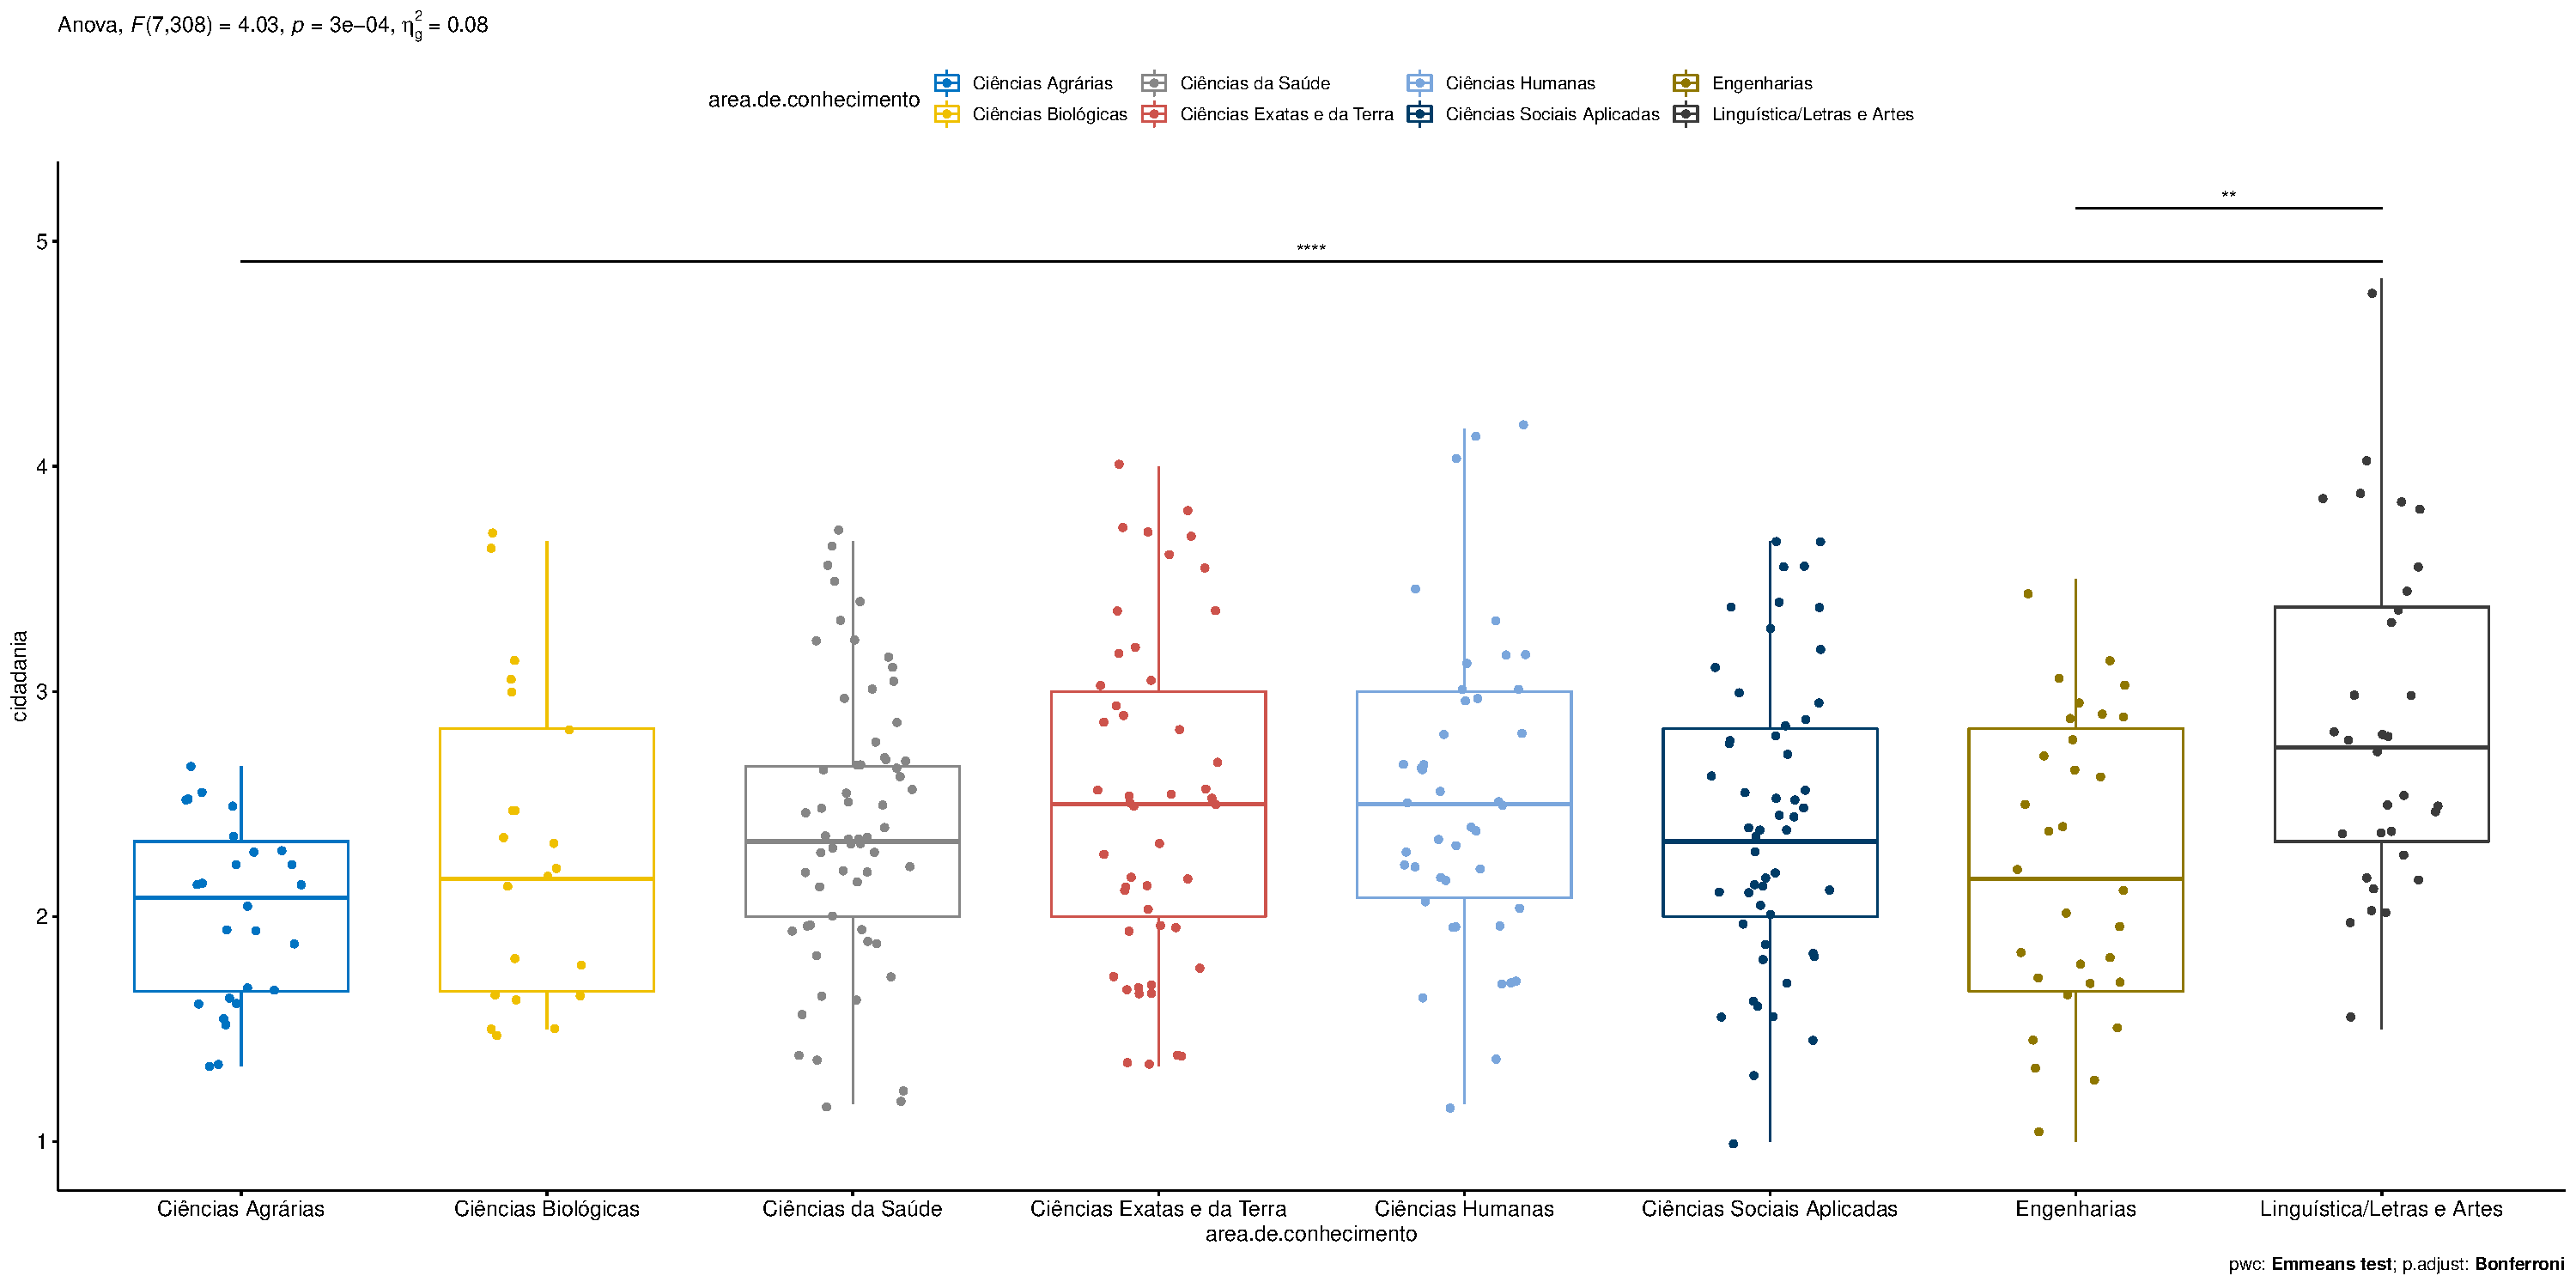
\includegraphics{factorialAnova_files/figure-latex/unnamed-chunk-34-1.pdf}

\hypertarget{references}{%
\subsection{References}\label{references}}

{[}1{]}: Blanca, M. J., Alarcón, R., Arnau, J., Bono, R., \& Bendayan,
R. (2017). Non-normal data: Is ANOVA still a valid option?. Psicothema,
29(4), 552-557.

{[}2{]}: Ghasemi, A., \& Zahediasl, S. (2012). Normality tests for
statistical analysis: a guide for non-statisticians. International
journal of endocrinology and metabolism, 10(2), 486.

{[}3{]}: Miot, H. A. (2017). Assessing normality of data in clinical and
experimental trials. J Vasc Bras, 16(2), 88-91.


\end{document}
